\input graphicx.tex

\font\huge=cmr16 at 24pt
\font\sc=cmcsc10 at 10pt

\def\indent{\hskip2em}
\def\vsep{\vskip1.5em\vfil}

\vsize=8.5in
\voffset=-0.25in

\setbox0=\vbox{
  \vskip-0.5in%
  \vbox to 0pt {\rlap{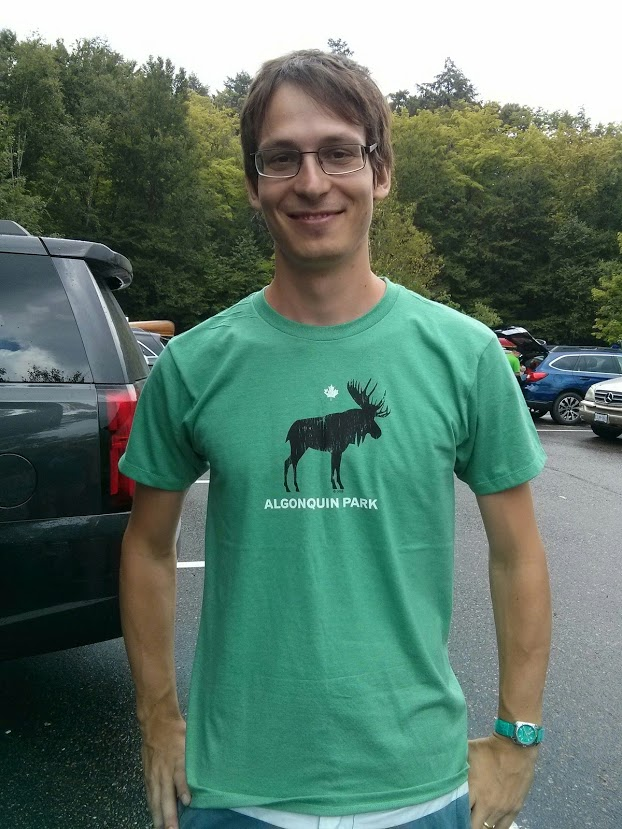
\includegraphics[trim={5cm 18cm 5cm 0},clip,width=4cm,keepaspectratio]{photo.jpg}}\vss}%
  \vskip0.5in%
  \vbox{%
    \hbox to \hsize {\huge \hfill RNDr. Jakub Daniel \hfill}%
    \vsep%
    \hbox to \hsize {\hfill Curriculum Vitae \hfill}%
  }%
}

\output={%
  \setbox255=\vbox{%
    \vbox to 1in {%
      \unvbox0%
    }%
    \vsep%
    \hrule%
      \vsep%
      \vbox to \vsize {\unvbox255\vfil}%
      \vsep%
    \hrule%
    \vsep%
    \hfil\the\pageno\hfil%
    \global\advance\pageno1%
  }%
  \shipout\box255%
}

\vbox{
  \halign{%
    \indent \hbox to 8em{#\hfil}&#\hfil\cr
    \multispan2{\bf Contact} \hfil\cr
    \cr

    Date of Birth:  & July 2, 1989\cr
    Residence:      & Veleslav\'\i{}nsk\'a 199/40 \cr
                    & 162 00 Praha 6 \cr
    \cr

    Phone:          & {\tt +420 723 739 962} \cr
    E-Mail:         & {\tt jakub.daniel@gmail.com} \cr
    GitHub:         & {\tt https://github.com/jakubdaniel} \cr
    Stack Overflow: & {\tt https://stackoverflow.com/users/1027321/jakubdaniel} \cr
  }
}
\vsep
\vbox{
  \halign{%
    \indent #\hfil\cr
    \multispan1{\bf Education} \cr
    \cr

    Ph.D. studies in Computer Science since 2013 (ongoing)\cr% (expected defence late 2017)\cr
    Faculty of Mathematics and Physics, Charles University in Prague\cr
    topic: Program Verification Using Abstraction and Logics\cr
    \cr

    RNDr. in Computer Science 2016 \cr
    Faculty of Mathematics and Physics, Charles University in Prague \cr
    %thesis: Analysis of Interface Automata with On-Demand Replication\cr
    state exam: \vtop{\hsize=15cm\noindent undecidable problems, graph algorithms, fast matrix multiplication, high-speed networking, polyhedral compilation, first-order theories and decision procedures} \cr\cr
    % Computer Science Foundations - undecidable problems
    % Software System Foundations - graph algorithms, fast matrix multiplication
    % Operating Systems - high speed networking
    % Programming Languages - polyhedral compilation
    % Formal Verification - first-order theories and decision procedures
    \cr

    Mgr. (MSc equivalent) in Computer Science 2011--2013 \cr
    Faculty of Mathematics and Physics, Charles University in Prague \cr
    %thesis: Analysis of Interface Automata with On-Demand Replication\cr
    \cr

    Bc. in Computer Science 2008--2011 \cr
    Faculty of Mathematics and Physics, Charles University in Prague \cr
  }
}
\vsep
\vbox{
  \halign{%
    \indent #\hfil\cr
    \multispan1{\bf Internship} \cr
    \cr

    Project: Verifying Liveness Properties of Infinite-State Systems \cr
    Embedded Systems Group, Fondazione Bruno Kessler, Trento, Italy (Sep - Dec 2015) \cr
  }
}
\vsep
\vbox{
  \halign{%
    \indent #\hfil\cr
    \multispan1{\bf Software} \cr
    \cr
    {\sc Bacon}: {\sc B}ehaviour {\sc a}bstraction for {\sc con}tainers \hfil\cr
    {\tt https://github.com/d3sformal/bacon.git} \cr
    \cr
    {\sc Panda}: {\sc P}redicate {\sc a}bstraction i{\sc n} {\sc d}ynamic {\sc a}nalysis \hfil\cr
    Started as Google Summer of Code project in 2013 \cr
    {\tt https://github.com/d3sformal/panda.git} \cr
    \cr
    {\sc Expressions} \cr
    Toy Haskell library for representing sorted expressions and (boolean) formul\ae{} in dependently-typed manner \cr
    {\tt https://github.com/jakubdaniel/expressions.git} \cr
    {\tt https://github.com/jakubdaniel/expressions-z3.git} \cr
  }
}
\vsep
\vbox{
  \halign{%
    \indent #\hfil\cr
    \multispan1{\bf Programming Languages} \hfil\cr
    \cr

    proficient: Haskell, C, C++, Java, Bash \cr
    standard: Javascript, PHP, SQL, (X)HTML, CSS, \TeX \cr
    basic knowledge: Python, C\#, Lisp, Prolog, ASM \cr
  }
}
\vsep
\vbox{
  \halign{%
    \indent #&\hskip1em#\hfil\cr
    \multispan1{\bf Skills} \hfil\cr
    \cr

    Version Control:    & {\tt git} (preferred), {\tt hg}, {\tt svn} \cr
    Packaging \& Build: & {\tt cabal}, {\tt make}, {\tt ant}, {\tt portage/ebuild} \cr
    Environment:        & {\tt unix} ({\tt linux}, {\tt bsd}), {\tt vim}, {\tt ssh}, {\tt tmux}, {\tt xmonad}, {\tt dwm} \cr
    Solvers:            & {\tt z3}, {\tt mathsat} \cr
  }
}
\vsep
\vbox{
  \halign{%
    \indent #\hfil\cr
    \multispan1{\bf Languages} \hfil\cr
    \cr

    Czech (native) \cr
    English (advanced spoken/written) \cr %(FCE awarded in 2007) \cr
    Spanish (passive) \cr
  }
}
\vsep
{
  \newcount\pubnum
  \pubnum=0
  \def\item{\cr\global\advance\pubnum by 1[\the\pubnum] &}
  \vbox{
    \halign{%
      \indent {\hsize=4em #\hfil}\hskip1em&{\advance\hsize by -7em \vtop{\parindent=0pt #}\hfil} \cr
      \multispan2{\bf Publications} \hfil\cr

      \item J. Daniel, A. Cimatti, A. Griggio, S. Tonetta, and S. Mover. Infinite-state Liveness-to-Safety via Implicit Abstraction and Well-founded Relations. Accepted for publication in Proceedings of CAV 2016. \cr

      \item J. Daniel and P. Parizek. {\sc Panda}: Simultaneous Predicate Abstraction and Concrete Execution. In Proceedings of the 11th Haifa Verification Conference, LNCS, vol. 9434, Nov 2015. \cr

      \item T. Ball and J. Daniel. Deconstructing Dynamic Symbolic Execution. In Proceedings of the 2014 Marktoberdorf Summer School on Dependable Software Systems Engineering, IOS Press, Jan 2015. \cr

      %\item J. Daniel and P. Par\'{\i}zek. Predicate Abstraction in Program Verification: Survey and Current Trends. Accepted for publication in Proceedings of ICCSW 2014 \cr
      \item J. Daniel and P. Parizek. Predicate Abstraction in Program Verification: Survey and Current Trends. In Proceedings of 2014 Imperial College Computing Student Workshop, OASIcs, vol. 43. \cr

      %\item J. Daniel, P. Par\'{\i}zek, and C. P\u{a}s\u{a}reanu. Predicate Abstraction in Java Pathfinder. In Proceedings of the Java Pathfinder Workshop 2013, ACM SIGSOFT Software Engineering Notes, 39(1) \cr
      \item J. Daniel, P. Parizek, and C. Pasareanu. Predicate Abstraction in Java Pathfinder. In Proceedings of the Java Pathfinder Workshop 2013, ACM SIGSOFT Software Engineering Notes, 39(1) \cr
      % Garbage item. Nothing to do with me!
      %\item T. Knap, J. Michelfeit, J. Daniel, P. Jerman, D. Rychnovsk\'{y}, T. Soukup, and M. Ne\v{c}ask\'{y}. ODCleanStore: A Framework for Managing and Providing Integrated Linked Data on the Web. In Proceedings of WISE 2012, LNCS, vol. 7651, Nov 2012.\cr
      %\item T. Knap, J. Michelfeit, J. Daniel, P. Jerman, D. Rychnovsky, T. Soukup, and M. Necasky. ODCleanStore: A Framework for Managing and Providing Integrated Linked Data on the Web. In Proceedings of WISE 2012, LNCS, vol. 7651, Nov 2012.\cr
    }
  }
}
\vsep
\vbox{
  \halign to \hsize {%
    \indent {\hsize=5em #\hfil}&{\hsize=5em #\hfil}\hskip1em& {#\hfil}\hskip1em& {#}\hfil \cr
    \multispan3{\bf Teaching Experience} \hfil\cr
    \cr

    Summer & '16, '17 & Recommended Programming Practices          & Charles University in Prague\cr
    Winter & '16      & Unix Administration                        & Charles University in Prague\cr
    Summer & '14, '15 & System Behaviour Models and Verification   & Charles University in Prague\cr
    Winter & '14      & Java                                       & Charles University in Prague\cr
    Winter & '13, '14 & Developing Applications for Mobile Devices & Charles University in Prague\cr
  }
}
\vsep
\vbox{
  \halign{%
    \indent \hbox to \hsize{\vtop{\parindent=0pt #}\hfil}&#\hfil\cr
    \multispan1{\bf Interests} \hfil\cr
    \cr

    category theory, functional programming, strong static typing, dependent types, formal verification, program analysis, computability, computational complexity, logic, satisfiability modulo theories, theorem proving, sailing, snowboarding
    \cr
  }
}

\bye
